\documentclass[11pt]{article}
\usepackage{ctex}  

\usepackage[margin=1in]{geometry}
\usepackage{amsfonts,amsmath,amssymb}
\usepackage[none]{hyphenat}
\usepackage{fancyhdr}
\usepackage{graphicx}
\usepackage{float}
\usepackage{subfigure}
\usepackage{pgfplots}
\usepackage{enumerate}
\usepackage[colorlinks,linkcolor=black]{hyperref}

\pagestyle{fancy}
\fancyhead{}
\fancyfoot{}
%\fancyhead[L]{\slshape \MakeUppercase{Place Title Here}}
\fancyhead[C]{\slshape 启智ROS机器人小组}
\fancyfoot[C]{\thepage}
\renewcommand{\footrulewidth}{0pt}

%\parindent 0ex
\setlength{\parindent}{0em}%段落首位缩进数
\setlength{\parskip}{0em}%调段间距
\renewcommand{\baselinestretch}{1.5}%调行间距

\begin{document}
	
\begin{titlepage}
\begin{center}
\vspace*{1cm}
\Large{\textbf{清华大学}}\\
\Large{\textbf{电子设计小学期}}\\
\vfill
\line(1,0){400}\\[1mm]
\huge{\textbf{预习报告}}\\[3mm]
\Large{\textbf{启智ROS机器人小组}}\\[1mm]
\line(1,0){400}
\vfill
\today \\
\end{center}
\end{titlepage}

\tableofcontents
\thispagestyle{empty}
\clearpage

\setcounter{page}{1}
\noindent
\section{产品调研}
\subsection{启智ROS机器人}
启智ROS机器人是一款为ROS机器人算法开发量身打造的机器人硬件平台,拥有硬件里程计、激光 测距雷达、立体视觉相机和语音输入输出阵列等一系列设备,完美适配ROS的TF、Navigation、 Actionlib和Pluginlib子系统。其硬件设备和已实现的功能介绍如下。
\begin{figure}[H] %H为当前位置,!htb为忽略美学标准,htbp为浮动图形
    \centering %图片居中
    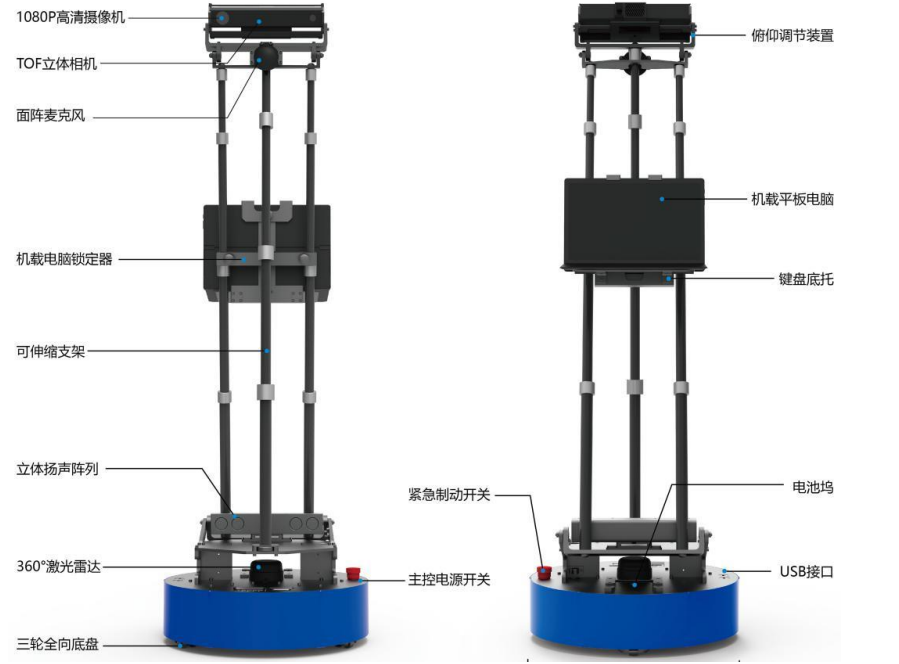
\includegraphics[width=0.5\textwidth]{5} %插入图片,[]中设置图片大小,{}中是图片文件名
    \caption{启智ROS机器人}
\end{figure}
\subsubsection{硬件配置}
\begin{enumerate}[$\bullet$]
    \item 激光雷达\\
    启智ROS机器人的底盘上安装了一枚红外激光雷达,激光雷达是地面移动机器人常用的一种传感器,其工作原理是用一个高速旋转的激光测距探头将周围
360°的障碍物分布状况测量出来。它能够很高效的检测出周围的障碍物分布,并可以通过SLAM技术进行机器人的自身定位,为机器人的移动导航提供数据基础。
\begin{figure}[H] %H为当前位置,!htb为忽略美学标准,htbp为浮动图形
    \centering %图片居中
    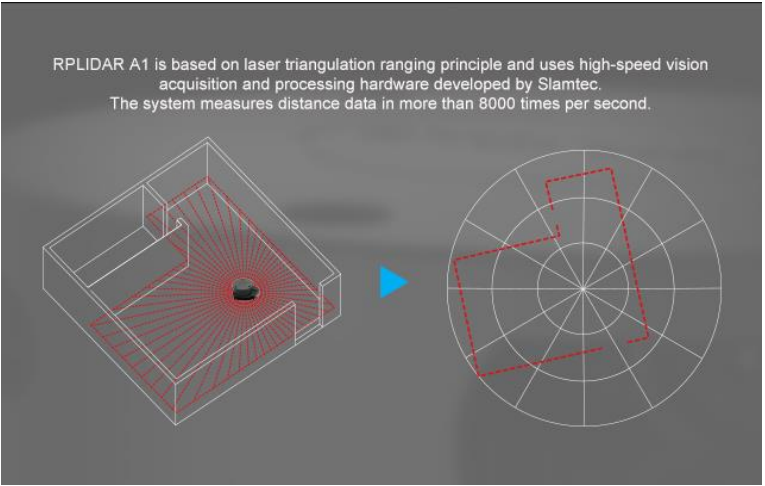
\includegraphics[width=0.5\textwidth]{7} %插入图片,[]中设置图片大小,{}中是图片文件名
    \caption{激光雷达原理图}
\end{figure}
    \item 底盘\\
    启智ROS机器人采用了三轮全向式移动底盘,相比传统的双轮差动底盘,拥有更多的自由度。全向底盘可以在不改变朝向的情况下往水平面上的任何方向移动,这在进行目标跟踪和运动避障时,可以减少机体位置调整的步骤,减少调节时间,提高执行效率。
    \item RGB-D相机\\
    启智ROS机器人的头部安装了一台RGB-D立体相机(Kinect)。立体相机可以输出RGB彩色视频流和Depth深度数据三维点云,借助OpenCV和PCL等开源图像库,可以对目标物进行准确识别和定位,以便进行后续的任务。
    \item 控制器\\
    启智控制器内部运行了启智 ROS 机器人专用固件,负责 PC
机于机器人之间的数据交互。PC
机将对底盘伺服电机的速度控制数据下发到启智控制器,由启智控制器通过半双工
RS485总线实时与 3
个底盘伺服电机通讯。启智控制器同时接收伺服电机的反馈信息,解析出它们当前的位置、电流信息与系统电压等信息汇总后发送到
PC 机。 
    \item 面阵麦克风\\
    启智 ROS
机器人头部安装了一枚面阵麦克风可以用于采集正前方的声音数据,可以用来接收人类的语音指令,并通过已有的语音识别和语音播报功能包,实现语音交流和控制。
    \item 无线路由器\\
    启智 ROS 机器人通过扩展一个无线路由器的方式来实现 WIFI
功能,利用此设备可以在PC端遥控控制机器人。
\end{enumerate}
\subsubsection{软件配置}
启智ROS机器人配有丰富的软件包和官方示例程序,可以很方便的实现电机、激光雷达、深度相机等设备的控制。
\begin{enumerate}[$\bullet$]
    \item slam建图------三维可视化平台Rviz\\
    激光雷达在软件层面已经高度封装,提供了一个名为``Rviz"的三维可视化平台,并提供了名为``map\_server''的
ROS
包,这个包用来保存和加载二维地图。只需要一行代码启动Rviz即可开始建图。最后会保存一份图片格式的地图和一份用于路径规划的栅格地图。
\begin{figure}[H] %H为当前位置,!htb为忽略美学标准,htbp为浮动图形
    \centering %图片居中
    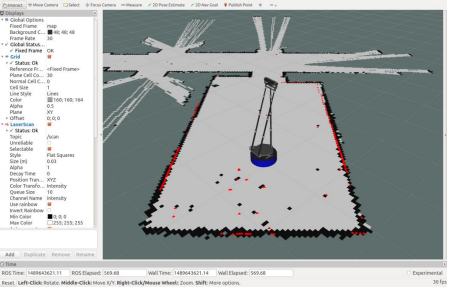
\includegraphics[width=0.5\textwidth]{8} %插入图片,[]中设置图片大小,{}中是图片文件名
    \caption{可视化三维平台Rviz}
\end{figure}
    \item navigation 自主避障------Move\_Base 包\\
    利用上面激光雷达建好的栅格地图,机器人就可以在其中寻找能够通过的空间区域并进行自主定位和路径规划。
MOVE\_BASE是导航系统里的核心中枢包,该软件包利用传感器信息生成一个代价地图,进行路径规划,并利用``蒙特卡洛自适应定位算法“(ACML)对机器人进行定位,计算出机器人当前应该执行的速度,发送到控制器里驱动机器人移动。
    \item 人脸检测------wpb\_home\_face\_detect\_3d\\
    基于RGB-D相机采集的图像,调用''wpb\_home\_face\_detect\_3d``来进行人脸定位。定位的结果同样用三维可视化平台Rviz显示。我们也可以编写自己的函数把这个结果存下来。
    \item 语音识别------科大讯飞云服务\\
    启智 ROS
机器人的配套源码里提供了一个使用科大讯飞云服务进行语音指令识别的
Package 包,可以联网后配合 Kinect2
的麦克风阵列完成语音识别功能。我们也可以编写自己的函数接收识别出来的字符串,给机器人控制信号,完成相应的动作。
\end{enumerate}
\section{可视化编程语言}
\subsection{可视化编程语言定义}
可视化编程语言(VPL)允许用户使用视觉表达、文本和图形符号的空间排列操作程序元素而不是通过代码来创建程序。\\
可视化编程语言的目的是使新手更容易进行编程,相比于传统的编程语言,它有如下三个方面的优势:
\begin{enumerate}[$\bullet$]
    \item 语法\\
    使用图标/块、表格和图表,试图减少甚至完全消除语法错误的可能性,自动生成代码以创建格式良好的程序。
    \item 语义\\
    可能会提供一些机制来揭示编程原语的含义,例如在一款名为``乐高机器人''的产品中,可视化编程语言将循环结构画成一个矩形框中,提示用户其中的内容会被反复执行;对于一条``移动''指令,则会在这条指令的方框中加上速度、方向选项,用户可以直接勾选而无需使用代码指定。
    \item 语用学\\
    支持研究程序在特定情况下的含义。这种级别的支持允许用户将使用 VPL
  创建的工件置于特定状态,以便探索程序将如何对该状态做出反应。例如:使用Thymio编程语言,用户可以将机器人置于特定状态,以查看它会如何反应,即激活哪些传感器。
\end{enumerate}
\subsection{可视化编程语言在机器人开发中的意义}
随着机器人在医疗、教育、服务、娱乐等众多领域的广泛使用,机器人应用开发平台的重要性逐渐凸显。目前大多数机器人应用开发平台都是基于文本语言编程的,
然而机器人行业的从业者往往是机械专业出生,对于代码、编程不是很熟悉,对于他们来说,使用代码编程难度大、复用率低、开发周期长、出错率高,因此不利于推广和使用。对于非计算机或者自动化专业的从业者来说,可视化编程就具有明显优势,
有利于简化机器人应用的开发,大幅提升机器人应用的开发效率。\\
此外,基于可视化编程的机器人在教育领域也发挥着重要作用,《中国STEM教育白皮书》指出,STEM是由科学、技术、工程、数学四个领域构成的。STEM教育鼓励学生主修科学、技术、工程和数学,有利于培养其科技理工素养。其中,机器人偏重技术与工程,但与四个领域均有关联。然而,机器人的开发涉及到预装环境,ROS操作系统,代码编写,算法库调用等较为专业的工程知识,对于没有经过训练的青少年来说,无疑是一个巨大的挑战。因此,对于刚入门的青少年,能够利用可视化编程语言进行开发,先快速地将机器人运行起来,以避免枯燥的理论学习浇灭了心中学习的热情,就显得尤为重要。
\subsection{可视化编程语言在机器人开发中的应用}
\begin{enumerate}
    \item Thymio II\\
    \textbf{Thymio II}是100
欧元价格范围内的教育机器人,由洛桑联邦理工学院(EPFL)与洛桑州艺术学院(ECAL)合作开发,苏黎世联邦理工学院(ETH)为其开发了一种纯可视化编程语言
。该机器人的主要特点是大量的传感器和执行机构、基于光和触摸的教育交互性、以及以图形和文本编程为特征的编程环境。\\
来自芬兰的教师Sharon
Marzouk在她的一篇文章``课堂机器人:激励自主学习和发现''中说道:对于
8-10 岁左右的学生来说,Thymio
是教授实验、技术、批判性思维、编程、发明、团队合作、设计、建筑\ldots{}\ldots{}的绝佳工具......我喜欢
\textbf{Thymio}
激发孩子们进入机器人技术并减少了编程的恐惧这一事实。\\
关于如何在课堂上使用 \textbf{Thymio} 进行教学的文章还有很多,正如 IEEE
所指出的那样,研究和新的 \textbf{Thymio} 项目正在不断进行。2020
年,\textbf{Thymio} 的教学设计得到了芬兰教育联盟的评估,主要评估了
\textbf{Thymio} 的课程一致性、教学法和可用性。最终 \textbf{Thymio}
获得了教学质量认证。
    \item 乐聚机器人\\
    \textbf{乐聚机器人}由乐聚(深圳)机器人技术有限公司研发,主要产品有AELOS娱乐版、教育版、专业版机器人和PANDO机器人。\\
其中AELOS教育版主要应用于中小学教育以及机器人培训机构。可为全球中小学生及机器人青少年爱好者提供人形机器人教育服务,该服务集硬件、编程软件、课程体系、教员培训、机器人竞赛平台于一体,提供steam及创新创客教育。\\
PANDO则是一款注重与人情感互动的机器人,也是乐聚第一款具有表情交互功能的产品。可拼装设计以及基于Blocky二次开发的机器人编程学习功能,加上18个自由度和新的步态算法,整体可玩性和趣味性进一步提升。\\
他们都可以使用可视化编程语言编程,推出不久便受到了很多青少年的欢迎,被广泛应用于``创客教育''、"stem教育"之中。\\
\begin{figure}[H] %H为当前位置,!htb为忽略美学标准,htbp为浮动图形
    \centering %图片居中
    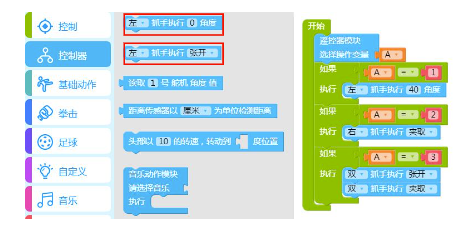
\includegraphics[width=0.5\textwidth]{6.PNG} %插入图片,[]中设置图片大小,{}中是图片文件名
    \caption{乐聚机器人的可视化编程语言}
\end{figure}
\end{enumerate}
\subsection{预期效果}
鉴于上述情况,本课题研究的是基于可视化编程语言的机器人开发平台,
主要围绕下面四个方面展开:
\begin{enumerate}
    \item 机器人可视化编程语言,计划基于QT搭建。
    \item 基于机器人可视化编程语言的代码自动生成算法,将界面上的模块``翻译''为ROS命令和函数调用指令。
    \item 除此之外,本组同学还计划为启智ROS机器人额外加装一个机械臂,该机械臂用单片机控制,以实现物品抓取等功能。硬件的连接关系如下图所示。
    \item 基于搭建好的平台要实现的功能有自主避障(路径规划),slam建图、人脸识别、目标跟踪、物体抓取、语音交互等,再通过这些功能构建不同的应用场景。
\end{enumerate}
\begin{figure}[H] %H为当前位置,!htb为忽略美学标准,htbp为浮动图形
    \centering %图片居中
    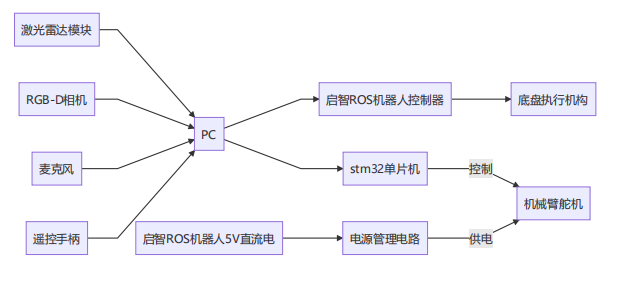
\includegraphics[width=0.5\textwidth]{9} %插入图片,[]中设置图片大小,{}中是图片文件名
\end{figure}
\section{电路框图 \& 电源管理电路 \& 数字系统流程图}
\subsection{目的}
在输入电压有波动和输出端负载有变化的情况下,为电子设备提供稳定的直流电源供电。
\subsection{性能指标}
\begin{enumerate}[$\bullet$]
    \item 稳压系数/电源电压调节率
    \item 输出电阻/负载调节流
    \item 输出纹波/电源纹波抑制比
    \item 环路稳定性、瞬态响应、效率
\end{enumerate}
\subsection{分类}
\begin{enumerate}[$\bullet$]
    \item 线性稳压电路
    \begin{figure}[H] %H为当前位置,!htb为忽略美学标准,htbp为浮动图形
        \centering %图片居中
        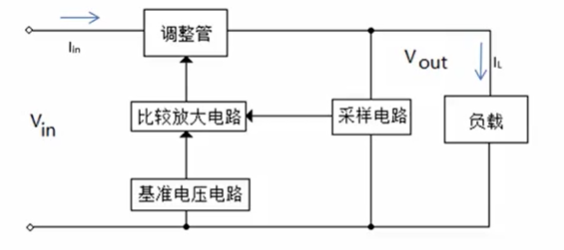
\includegraphics[width=0.5\textwidth]{10.PNG} %插入图片,[]中设置图片大小,{}中是图片文件名
    \end{figure}
    效率低
    \item 开关稳压电路
    \begin{figure}[H] %H为当前位置,!htb为忽略美学标准,htbp为浮动图形
        \centering %图片居中
        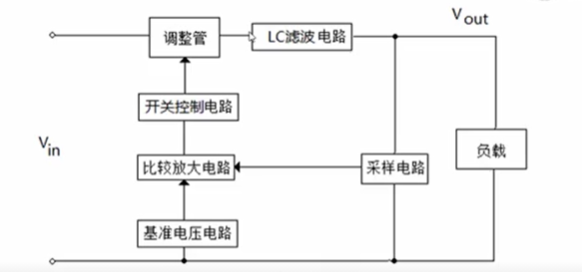
\includegraphics[width=0.5\textwidth]{11.PNG} %插入图片,[]中设置图片大小,{}中是图片文件名
    \end{figure}
    波纹电压大,但效率高,数字电路中一般采用这种。
\end{enumerate}
\subsection{WEBENCH仿真}
\begin{enumerate}[$\bullet$]
    \item 电路框图\\
    PC机和启智ROS机器人,PC机和stm32都可以通过usb直接连接,不需要设计接口电路。\\
stm32输出的控制信号为3.3V,机械臂的MG996舵机需要的PWM波高电平为5V,需要电平转换电路,设计如下。
\begin{figure}[H] %H为当前位置,!htb为忽略美学标准,htbp为浮动图形
    \centering %图片居中
    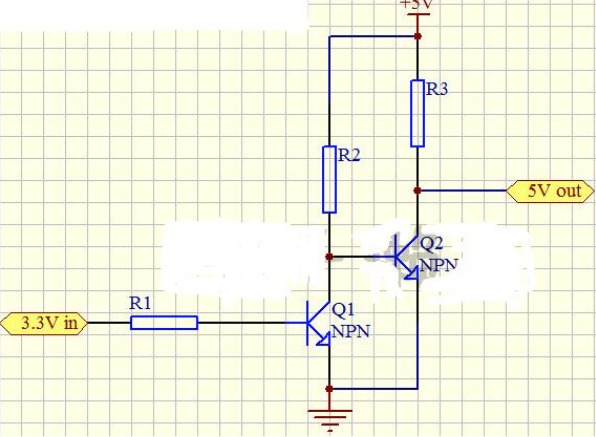
\includegraphics[width=0.5\textwidth]{12.PNG} %插入图片,[]中设置图片大小,{}中是图片文件名
\end{figure}
这个电路是通过三极管来实现3.3V电平转换成5V电平。当3.3V系统输入高电平时,三极管Q1导通,Q2截止,5V通过电阻R3输入到5V系统,也是高电平。当3.3V系统输入低电平时,三极管Q1截止,那么Q2导通,Q2集电极被拉低到低电平,那么输入到5V系统的就为低电平。这样输入输出就符合了5V电平要求。\\
我们使用的电池是12V电池,需要转为5V,来给舵机供电,设输入电压的变化范围为11V到13V, MG996舵机需要的供电电压为5V,空载转动所需电流为120mA,堵转电流为300mA,以带载4部舵机 计算,每部舵机都被堵转计算,所需最大电流为1.2A。电路设计如下。
\begin{figure}[H] %H为当前位置,!htb为忽略美学标准,htbp为浮动图形
    \centering %图片居中
    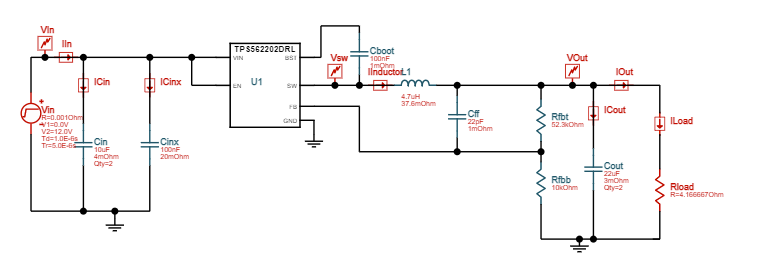
\includegraphics[width=0.5\textwidth]{13.PNG} %插入图片,[]中设置图片大小,{}中是图片文件名
\end{figure}
    \item 启动时\\
    \begin{figure}[H] %H为当前位置,!htb为忽略美学标准,htbp为浮动图形
        \centering %图片居中
        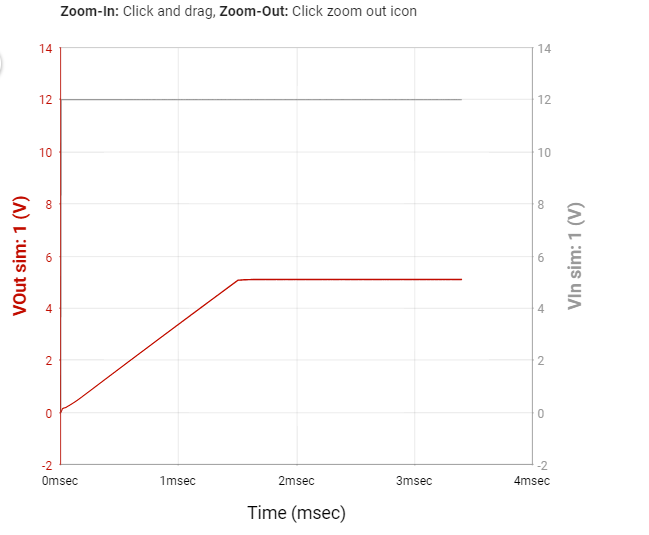
\includegraphics[width=0.5\textwidth]{14.PNG} %插入图片,[]中设置图片大小,{}中是图片文件名
    \end{figure}
    \begin{figure}[H] %H为当前位置,!htb为忽略美学标准,htbp为浮动图形
        \centering %图片居中
        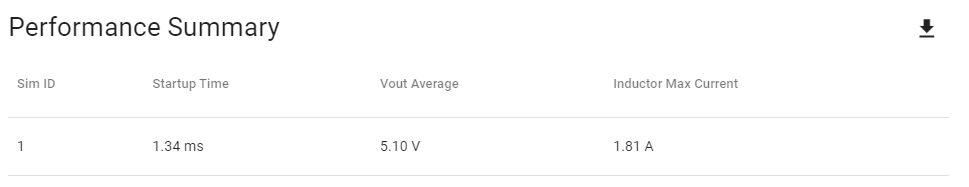
\includegraphics[width=0.5\textwidth]{15.PNG} %插入图片,[]中设置图片大小,{}中是图片文件名
    \end{figure}
    \item 输入电压变化时
    \begin{figure}[H] %H为当前位置,!htb为忽略美学标准,htbp为浮动图形
        \centering %图片居中
        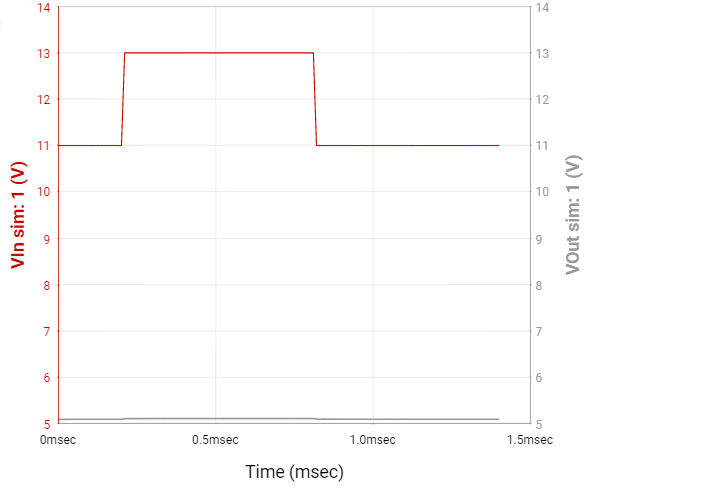
\includegraphics[width=0.5\textwidth]{21.PNG} %插入图片,[]中设置图片大小,{}中是图片文件名
    \end{figure}
    \begin{figure}[H] %H为当前位置,!htb为忽略美学标准,htbp为浮动图形
        \centering %图片居中
        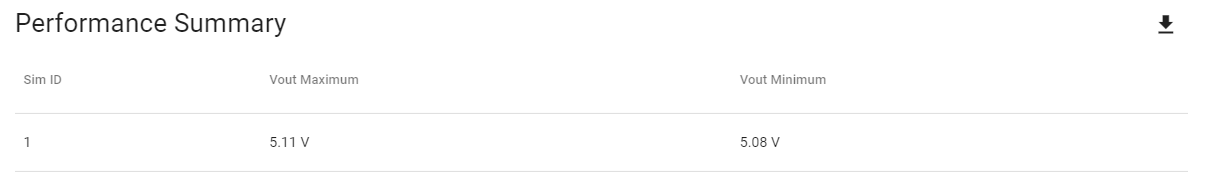
\includegraphics[width=0.5\textwidth]{22.PNG} %插入图片,[]中设置图片大小,{}中是图片文件名
    \end{figure}
    \item 负载变化时\\
    \begin{figure}[H] %H为当前位置,!htb为忽略美学标准,htbp为浮动图形
        \centering %图片居中
        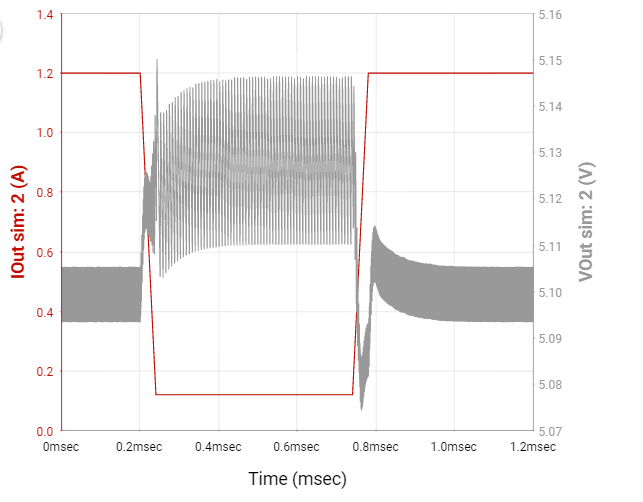
\includegraphics[width=0.5\textwidth]{16.PNG} %插入图片,[]中设置图片大小,{}中是图片文件名
    \end{figure}
    \item 稳态时\\
    \begin{figure}[H] %H为当前位置,!htb为忽略美学标准,htbp为浮动图形
        \centering %图片居中
        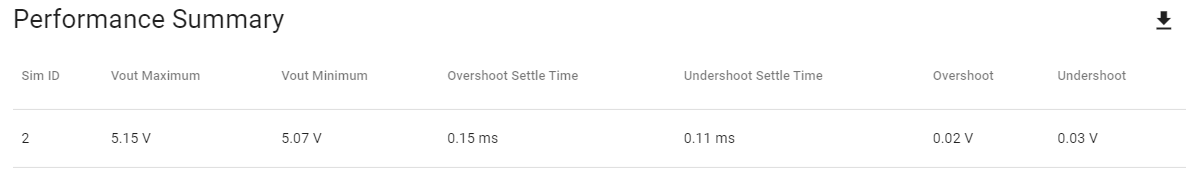
\includegraphics[width=0.5\textwidth]{20.PNG} %插入图片,[]中设置图片大小,{}中是图片文件名
    \end{figure}
    \begin{figure}[H] %H为当前位置,!htb为忽略美学标准,htbp为浮动图形
        \centering %图片居中
        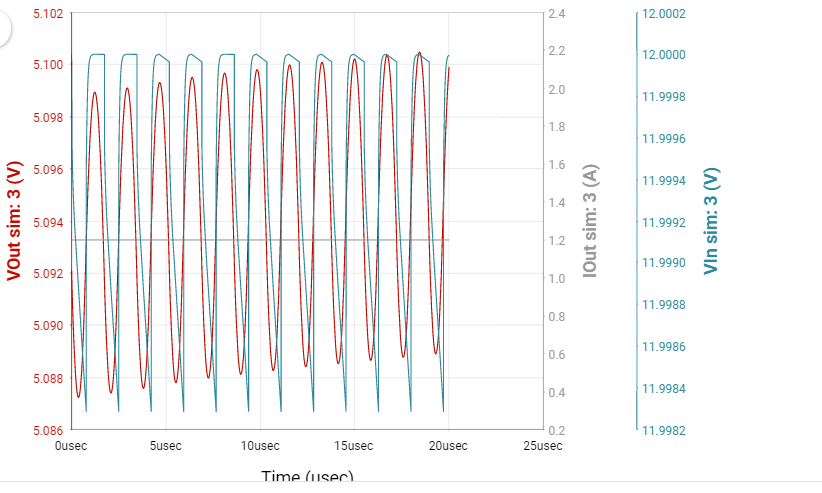
\includegraphics[width=0.5\textwidth]{17.PNG} %插入图片,[]中设置图片大小,{}中是图片文件名
    \end{figure}
    \begin{figure}[H] %H为当前位置,!htb为忽略美学标准,htbp为浮动图形
        \centering %图片居中
        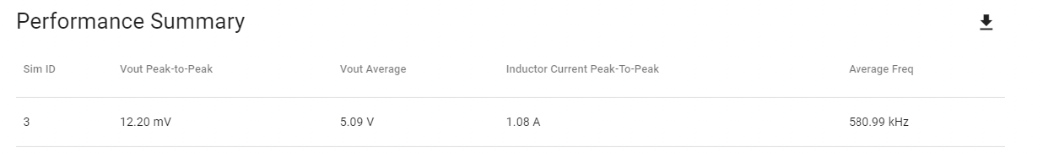
\includegraphics[width=0.5\textwidth]{23.PNG} %插入图片,[]中设置图片大小,{}中是图片文件名
    \end{figure}
    可以看到,在输入电压变化的情况下,输出电压在5.08V至5.11V之间变化,在负载变化时,负载电流在 0.1A至1.2A大范围内变化时,输出电压在5.07V至5.15V之间变化,变化范围很小。稳态时有一定波纹电 压,在可接受的范围内。\\
    综上,该电源管理电路满足设计要求。
\end{enumerate}
\subsection{数字系统流程图}
\begin{figure}[H] %H为当前位置,!htb为忽略美学标准,htbp为浮动图形
    \centering %图片居中
    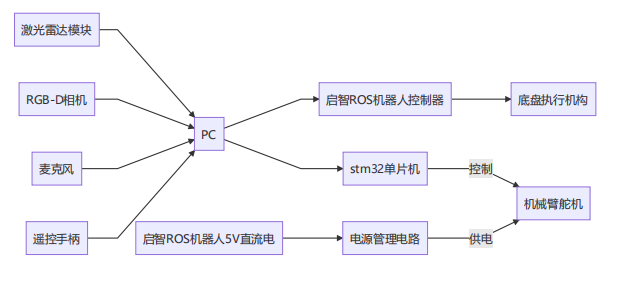
\includegraphics[width=0.5\textwidth]{18.PNG} %插入图片,[]中设置图片大小,{}中是图片文件名
\end{figure}
\section{机械臂调研}
\subsection{应用现状及功能需求}
机械臂抓取是服务机器人与环境进行交互的重要途经,机械臂具有独特的操作灵活性,在工业界以及服务业都有广泛应用。机械臂是一个复杂的系统,其建模模型具有多样性和不确定性。需要针对性的规划机械臂空间运动轨迹。\\
面向服务的机器人以视觉为传感器,根据用户指令识别并抓取指定物体,通常需要构建模型库,实现物体识别,计算六自由度的位置与姿态,生成抓取状态,规划运动路径,通过软件和硬件共同控制机械臂的运动。本项目针对餐厅这一特定场景进行设计,一定程度上简化了模型。\\
本项目在原有机器人的基础上添加机械臂,以实现更多功能,如上菜、添水、加餐具等功能。而多样的需求对物品的准确抓取带来挑战,不同物体具有不同的外形以及不同的硬度,因此机械臂需要针对餐厅的各个物品做出相应动作。同时机械臂应准确识别和定位不同物体,并通过控制不同关节,到达指定物体位置。\\
下面展示了一些具有先进机械臂的服务机器人,智能程度较高且应用场景较为广泛。
\begin{figure}[H]
    \centering
    \subfigure{
        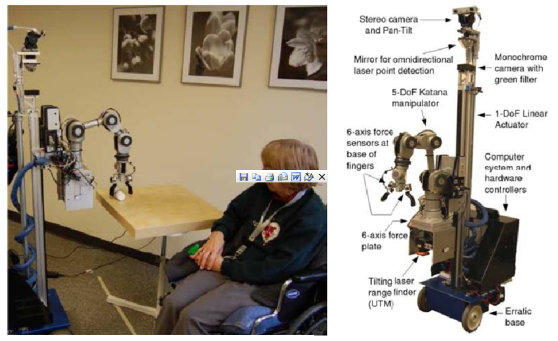
\includegraphics[width = 0.3\textwidth]{1.png}
    }
    \hspace{1cm}
    \subfigure{
        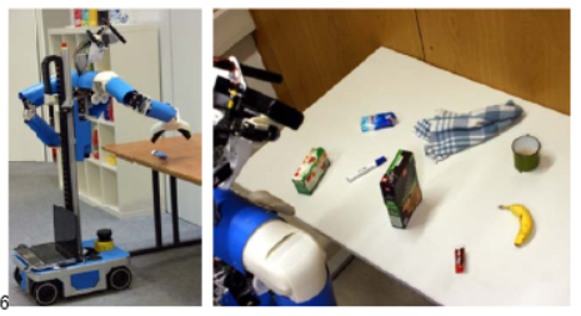
\includegraphics[width = 0.3\textwidth]{2.png}
    }
\end{figure}
\begin{figure}[H] %H为当前位置,!htb为忽略美学标准,htbp为浮动图形
    \centering %图片居中
    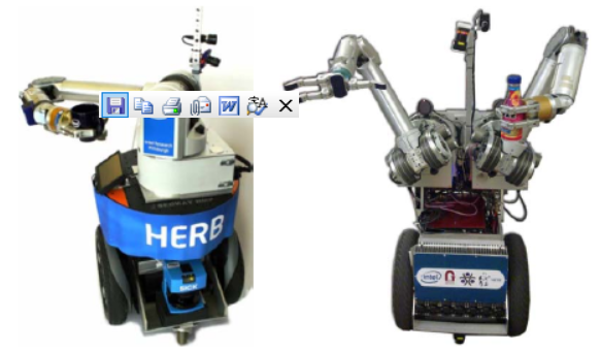
\includegraphics[width=0.5\textwidth]{3} %插入图片,[]中设置图片大小,{}中是图片文件名
    \caption{机械臂图}
\end{figure}
\subsection{六轴机械臂简介}
六轴机械臂是现代较为常见的机械臂,由X移动、Y移动、Z移动、X转动、Y转动、Z转动六个自由度组成,动作灵活,位置精度高,通用性强,能适应多种场景和环境。\\
在机械臂运动学研究领域,正向运动学和逆向运动学是基础且关键的问题。建立各个旋转关节坐标系并定义机械臂初始位置,如图所示,使用逆运动学方法求解后在仿真软件进行验证。本项目采用较为成熟的机械臂平台,因此不必陷入复杂且陌生的机械设计。
\begin{figure}[H] %H为当前位置,!htb为忽略美学标准,htbp为浮动图形
    \centering %图片居中
    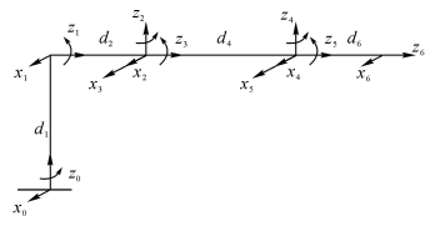
\includegraphics[width=0.5\textwidth]{4} %插入图片,[]中设置图片大小,{}中是图片文件名
    \caption{坐标轴图}
\end{figure}
\subsection{机械臂设计方案}
本项目使用六轴机械臂,将机械臂外接到原有机器人平台上,实现功能扩展。使用电源管理电路为机械臂的舵机供电,使用stm32单片机对六个舵机进行控制。\\
在收到顾客发出的指令后,机器人对指令进行解析,判断需要抓取的物体及后续动作。使用摄像头识别出具体物品,如盘子、水杯等。对其定位后,展开机械臂进行抓取,并将物品移动到指定位置。
\section{应用探索}
\subsection{餐厅服务机器人}
\subsubsection{应用现状及功能需求}
世界上第一台餐厅服务机器人于1999年由加拿大设计而成,其具有通过语音识别与客户交互点菜的功能;在2006年与2012年,香港两次引进餐厅服务机器人,这些机器人功能丰富,可以完成送菜点餐、迎宾收账等餐厅服务基础功能。截止目前,餐厅机器人能够完成与客人的简单交互,如打招呼、点菜、上菜、收盘等简单互动,但这些互动程度仍然不够,我们需要通过模块化编程并将多种功能共同封装为整体,从而完成设计一个可互动性强、人性化服务的餐厅服务机器人。
\subsubsection{功能设计}
使用已经封装好的编程模块,根据顾客或服务员在机器人平台上所下的不同指令完成对应的服务操作。
\begin{enumerate}
    \item 点菜\\
    界面首先识别客户在机器人平台上的点菜需求(可加入语音识别),此时可以通过连接APP完成点菜的直接操作,抑或通过语音识别或手写输入等方式将点菜信息全部传进机器人平台。可在每个菜品尾部设置问询键,顾客点击后机器人可通过语音功能完成对此菜品的介绍。
    \item 等餐环节的娱乐互动\\
    当顾客在等餐环节时选择“娱乐互动”时,机器人将进入已封装好的有关“娱乐互动”的模块,可供顾客选择“歌曲伴奏”或者“新闻播放”等功能,并能够通过连接APP来完成更多信息的查询。
    \item 上菜\\
    这一环节由后厨或服务员进行点击,在相应菜品被选中后,机器人通过机械臂完成对餐盘的抓取,并同时播报与当前所上菜品有关的注意事项或者用餐方式。
    \item 用餐服务\\
    如果顾客在用餐过程中需要添水,只需点击相应的指令,然后将水杯放入机械臂的抓取部位,由机器人自动完成添水服务,与此类似的功能还有加纸巾、加餐具等抓取功能,都可通过相应模块的调用来完成机械臂的具体抓取操作。
    \item 迎宾与送客\\
    可以利用VSLAM三维重建来完成对室内位置信息的三维重建,通过激光雷达的SLAM感知空间中与顾客的位置信息,从而可以在顾客进入餐厅与离开餐厅时完成自动跟随。同时可以根据人脸识别功能来记录进入餐厅顾客的实时人数,并在检测进店与出店时语音播报“欢迎光临”与“谢谢惠顾”等,同时完成用餐座位的引导。
\end{enumerate}
\subsection{测温机器人}
\subsubsection{背景介绍}
2020年初,一场突如其来的新冠疫情席卷全球,为了应对病毒的袭击,人类从疫苗研发、政策研究、辅助仪器等入手,开展了一场人类和病毒的军备竞赛。智能测温仪器机器人(我愿称之为“克毒一号”)的理念就来自于和病毒斗智斗勇的过程。在新冠疫情防控流程中,于前期发现感染者并及时治理至关重要,发现感染者的一个重要措施就是及时强制测温。出于对及时性和强制性的考虑,自动测温机器人可踪合软件和硬件,提高测温的速度和精准度,并可扩展处测温外的其他功能,实现全方位的智能化服务。
\subsubsection{功能设计}
\begin{enumerate}
    \item 自动导航测温功能\\
    测温功能是本机器人的核心功能。我通过观察平时楼道里的测温机器,发现尽管有精准的测温功能,但很多同学都对这些仪器视而不见,不测温或者随便一测就进楼了。这样就会产生很大的问题:体温有问题的同学可能没有被发现,而体温没问题的同学反复被测温,就会导致资源浪费以及时间浪费。为了解决传统测温仪器的无效性,我们希望充分利用机器人的灵活移动特点,实现点对点的自动导航测温。首先是在场景中放置机器人,根据VSLAM三维重建建立室内的人物分布模型,机器人在平板上存储每个人的体温信息,未被测温者放在队列首位,机器人不停移动,根据人物的位置信息导航,到测温者前测温,记录测温数据,机器人持续运动,直到房间内人们的体温被测完之前。
    \item 语音功能\\
    在我看来,一个智能化的机器人,需要会动、会看、会听、会说。会听和会说就是语音功能,主要是机器人语音播报和人声声控功能。机器人语音播报功能能够通过外接扩音设备,如果测温后发现被测者体温异常,可以根据需要播放报警音乐,警示房间里的其他人。人声声控功能则是根据需要利用语音识别模块识别语音指令,在机器人内部内置指令,从而遥控机器人动作。语音功能的添加大大增加了机器人的灵活性。
    \item 人脸识别功能\\
    传统的测温器是通过刷学生卡确定被测者身份,为了实现机器人“会看”的功能,我们希望能够利用机器人上的平板识别人脸,确定身份,免去了刷学生卡的步骤,更加智能化。配合机器人的自动跟随功能,实现“不知不觉”中就完成了测温。
    \item 网络发射功能\\
    网络信息发射功能就是通过无线局域网实现与中心数据库的互联。当机器人完成测温后,被测者的数据被传输到学校的数据中心。如果被测者的体温异常,数据中心会迅速收到消息,并发出行动。基于网络功能,还可以二次开发app,让被测者随时能够察看自己的体温情况和近日行踪,也有利行程回溯。
    \item 自动跟随功能\\
    自动跟随功能是自动导航功能的附加功能,在实现自动导航的基础之上,机器人会优先测量队列上的队首,如未成功测量,机器人会持续跟随被测者。当被测者离开房间时,队列更新;当被测者未离开房间,机器人会持续跟随被测者,若被测者故意躲避机器人或遮挡脸部不测温,机器人不会停止测量下一个人,利用被测者的羞耻心理督促他们测量体温。
\end{enumerate}

\begin{thebibliography}{99} 
    \bibitem{ref1}National Oceanic and Atmospheric Administration (26 February 2021). "What is LIDAR". oceanservice.noaa.gov. US Department of Commerce. Retrieved 15 March 2021.
    \bibitem{ref2}\href{https://blog.csdn.net/ycy_dy/article/details/78353894}{三轮全向移动底盘运动学解析}
    \bibitem{ref3}词条 \href{https://en.wikipedia.org/wiki/Kinect}{Kinect}
    \bibitem{ref4}启智ROS版实验指导书
    \bibitem{ref5}词条 \href{http://wiki.ros.org/amcl}{蒙特卡洛自适应定位算法}
    \bibitem{ref6}词条 \href{http://wiki.ros.org/move_base/move_base-1}{ROS move \_ base}
    \bibitem{ref7} Jost, Beate; Ketterl, Markus; Budde, Reinhard; Leimbach, Thorsten (2014). "Graphical Programming Environments for Educational Robots:
    Open Roberta - Yet Another One?". 2014 IEEE International Symposium on Multimedia. pp
    \bibitem{ref8}Repenning, Alexander (2017). "Moving Beyond Syntax: Lessons from 20 Years of Blocks Programing in AgentSheets". Journal of Visual
    Languages and Sentient Systems.
    \bibitem{ref9} \href{https://robohub.org/classroom-robotics-motivating-independent-lear
    ning-and-discovery/}{Classroom robotics: Motivating independent learning and discovery}
    \bibitem{ref10}"Education Alliance Finland". Catalog of certified products. Retrieved 12 May 2020.
    \bibitem{ref11}乐聚机器人在73届教育装备展获高关注 .凤凰网
    \bibitem{ref12}CES 2018,中国机器人整装待发! 新浪科技
    \bibitem{ref13}姜宏超,刘士荣,张波涛.六自由度模块化机械臂的逆运动学分析[J].浙江大学学报(工学版),2010,44(07):1348-1354.
    \bibitem{ref14}孙亮,马江,阮晓钢.六自由度机械臂轨迹规划与仿真研究[J].控制工程,2010,17(03):388-392.
    \bibitem{ref15}马江. 六自由度机械臂控制系统设计与运动学仿真[D].北京工业大学,2009.
    \bibitem{ref16}蒲睿.餐厅服务机器人设计[J].软件导刊,2015,14(07):85-87.
    \bibitem{ref17}苏业环,任军.智能送餐机器人设计[J].科技创新与应用,2018(07):32-34.
    \bibitem{ref18}周陆洲.餐厅服务机器人的应用分析[J].科技风,2015(15):122-123.
    \bibitem{ref19}孙晓刚, 李云红. 红外热像仪测温技术发展综述[J]. 激光与红外, 2008, 38(002):101-104.
    \bibitem{ref20}周广兵. 一种智能消毒防疫机器人:, CN111110896A[P]. 2020.
\end{thebibliography}

\end{document}
